\qns{RLC Circuit}
\qcontributor{Kyle Tanghe, Damanic Luck}

In this question, we will take a look at an electrical systems described by second-order differential equations and analyze it in the phasor domain. Consider the circuit below where $\tilde{V_{\text{s}}}$ is a sinusoidal signal, $L = \SI{1}{\milli\henry}$, and $C = \SI{1}{\nano\farad}$:

\begin{center}
		\begin{circuitikz}[scale=0.8]
			\draw (0,4) 
			to [sV, l_= $\tilde{V_s}$] (0,0)
			(0,4)
			to [R = $R$,v=$\tilde{V_R}$] (4,4)
			to [L = $L$,v=$\tilde{V_L}$] (8,4)
			to [short] (10,4)
			to [C = $C$,v=$\tilde{V_C}$] (10,0)	
			to [short] (0,0);
		\end{circuitikz}
	\end{center}
\begin{enumerate}
	
    \qitem \textbf{Transform the circuit into the phasor domain.}
    
\sol{

\begin{align*}
Z_R &= R \\ 
Z_L &= j\omega L \\
Z_C &= \frac{1}{j\omega C}
\end{align*}

}

\qitem \textbf{Solve for the transfer function $H_C(\omega)=\frac{\widetilde{V}_C}{\widetilde{V}_{\text{s}}}$ in terms of $R$, $L$, and $C$.}

\sol{

$\widetilde{V}_C$ is a voltage divider where the output voltage is taken across the capacitor.
\begin{align*}
\widetilde{V}_C&=\frac{Z_C}{Z_R+Z_L+Z_C}\widetilde{V}_{\text{s}}, \\
H_C(\omega)&=\frac{Z_C}{Z_R+Z_L+Z_C} = \frac{\frac{1}{j\omega C}}{R+j\omega L+\frac{1}{j\omega C}}.
\end{align*}
Multiplying the numerator and denominator by $j\omega C$ gives
\[H_C(\omega)=\frac{1}{(j\omega)^2LC+j\omega RC+1}\]

}

\qitem \textbf{Solve for the transfer function $H_L(\omega)=\frac{\widetilde{V}_L}{\widetilde{V}_{\text{s}}}$ in terms of $R$, $L$, and $C$.}

\sol{

$\widetilde{V}_L$ is a voltage divider where the output voltage is taken across the inductor.
\begin{align*}
\widetilde{V}_L&=\frac{Z_L}{Z_R+Z_L+Z_C}\widetilde{V}_{\text{s}}, \\
H_L(\omega)&=\frac{Z_L}{Z_R+Z_L+Z_C} = \frac{j\omega L}{R+j\omega L+\frac{1}{j\omega C}}.
\end{align*}
Multiplying the numerator and denominator by $j\omega C$ gives
\[H_L(\omega)=\frac{(j\omega)^2LC}{(j\omega)^2LC+j\omega RC+1}\]

}

\qitem \textbf{Solve for the transfer function $H_R(\omega)=\frac{\widetilde{V}_R}{\widetilde{V}_{\text{s}}}$ in terms of $R$, $L$, and $C$.}

\sol{

$\widetilde{V}_R$ is a voltage divider where the output voltage is taken across the resistor.
\begin{align*}
\widetilde{V}_R&=\frac{Z_R}{Z_R+Z_L+Z_C}\widetilde{V}_{\text{s}}, \\
H_R(\omega)&=\frac{Z_R}{Z_R+Z_L+Z_C} = \frac{R}{R+j\omega L+\frac{1}{j\omega C}}.
\end{align*}
Multiplying the numerator and denominator by $j\omega C$ gives
\[H_R(\omega)=\frac{j\omega RC}{(j\omega)^2LC+j\omega RC+1}.\]

}

\qitem \textbf{Sketch the Bode plots of $H_C(\omega)$, $H_L(\omega)$, and $H_R(\omega)$ when $R =\SI{2}{\kilo\ohm}$.}
\meta
{Emphasize that students factor the numerator and denominator of their transfer function so its easier to plot. This means students should rearrange their transfer function into rational transfer function form. We can plot by noticing that poles ($w_{pn}$) and zeros ($w_{zn}$) appear in the denominator and numerator, respectively, and constant (K) in this form: 
\[K \cdot \frac{(j\omega)^{z0} \cdot \Pi_{k=1}^n(1 \pm j \frac{\omega}{\omega_{zk}})}{(j\omega)^{p0} \cdot \Pi_{k=1}^n(1 \pm j \frac{\omega}{\omega_{pk}})} \] 
Also go over why we can superimpose each component's individual bode plot and "add" it up together at the end.
% Poles are out of scope for 16B This semester. Even though we have 2nd order filters, Students only need to know how to make bode plots out of a transfer function. There is more nuance than this for 2nd or higher order filters, but it should be out of scope for this class. (This is the original text, commenting it out to write new explanation.)

    % It might be good to mention that for the first to parts of part e, even though we have 3 circuit components, they're set up in series such that the filter is like a first order filter with $Z_R Z_L$ as the first impedence, and $Z_C$ as the second impedence, so it behaves closer to a first order filter.
}


    \sol{
    $H_C(\omega)$:

    Let's look at the poles. It is a second order transfer function of the form $\left(\frac{j\omega}{\omega_c}\right)^2+j\omega \frac{2\xi}{\omega_c}+1$, where $\omega_c = \frac {1} {\sqrt {LC}} =  \frac {1}{\sqrt{10^{-3}10^{-9}}} = 10^6$. There are two frequency terms in the denominator so there are two poles.
    This means that there are 2 poles at $\omega_c = 10^6$.
    
    Zeros:
    
    Since the numerator has no frequency terms, there are no zeros.
    
    We have 2 poles and no zeros, which means that this will be a low pass filter with a cutoff frequency of $\omega = 10^6$, with a -20 dB/decade rolloff \textit{per} pole. This means we have a -40 db/decade rolloff at $\omega=10^6$.
     
    To find the magnitude in the flatband for a low pass filter, we look at the magnitude when all frequency terms are 0. For this filter, we just get a magnitude of $\frac{1}{1} = 1$, or 0 dB. 
    
    % To find the magnitude in a filter, we look at the magnitude when all frequency terms are 0. For this filter, we get a magnitude of $\frac{1}{1} = 1$.
    
    % Similarly, if we take a the limit of frequency to $\infty$, we get a magnitude of $\frac{1}{\omega^2} = 0$
    
    To find the cutoff frequency, we need to set this into the rational transfer function form so that we can easily solve for $H_C(j\omega)= \frac{1}{\sqrt{2}}$. In.other words, we can model it in the form below to later pattern match what our cutoff frequency is .
    \[(\frac{1}{1 + \frac{j\omega}{\omega_c}})^2 = \frac{1}{(\frac{j\omega}{\omega_c})^2 + j\omega \frac{2E}{\omega_c} + 1}\] 
    where $\omega_c$ is our cutoff frequency and $E$ is an expression involving $R$, $C$, and $L$. In this form, we can see that $\omega_c = \sqrt{1/LC} = 10^6$
    
    %As for phase, the two poles will cause a phase shift starting at $10^5 \si{\radian\per\second}$ at a rate of $\frac{\ang{-90}}{\text{dec}}$ ($\frac{\ang{-45}}{\text{dec}}$ per pole) until a decade past the corner frequency. This results in the Bode plot below.
    
    As for phase, the cut off frequency at $\omega_c = 10^6$ will cause a phase shift starting at $10^5 \omega$ (one decade before $\omega_c$) until a decade $10^7 \omega$ (one decade after $\omega_c$) past the cutoff frequency. This results in the Bode plot below.

      \begin{figure}[H]\centering
  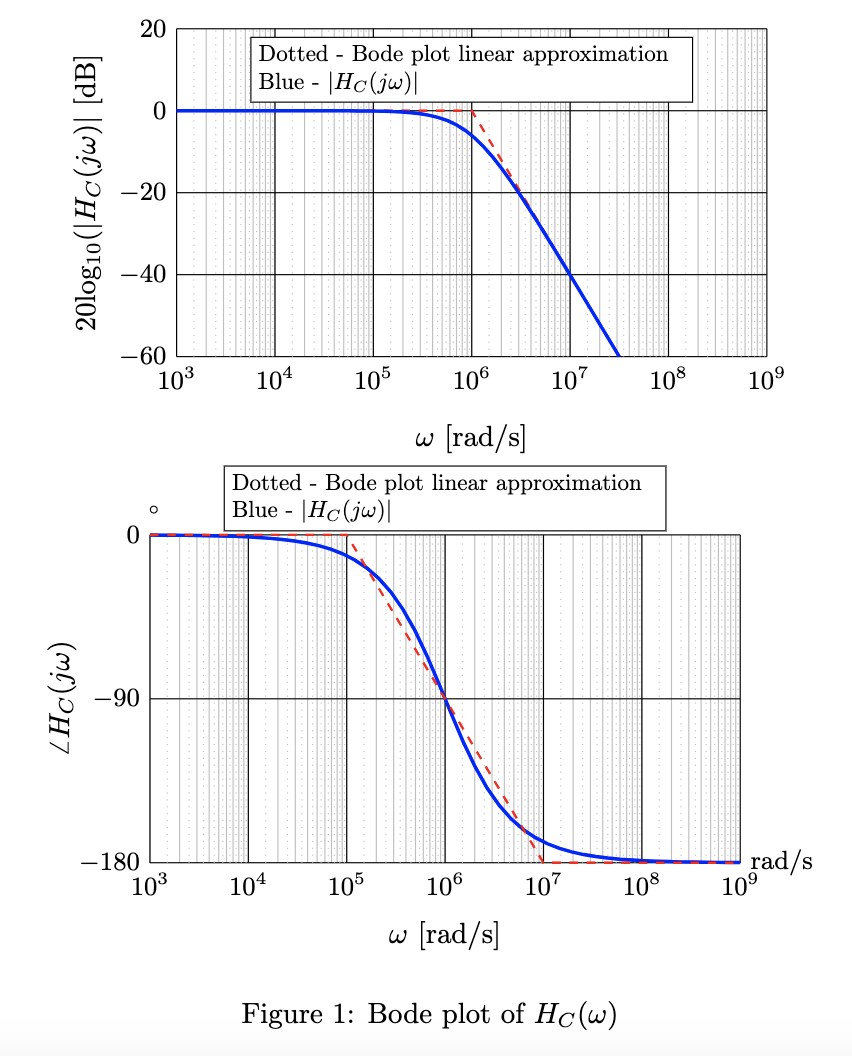
\includegraphics[width=0.8\textwidth]{\bank/transfer/figures/hc.png}
  % \caption{Bode plot of $H_C(\omega)$}
   \end{figure}
  % \begin{figure}[H]
    \centering
    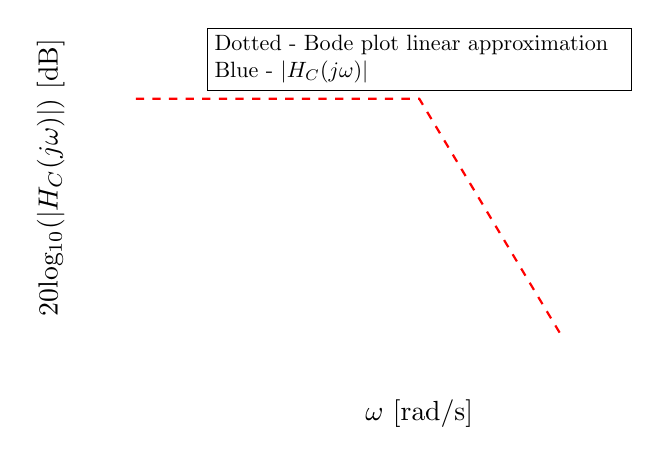
\begin{tikzpicture}[
        gnuplot def/.append style={prefix={}},
    ]
     \tikzset{
     semilog lines/.style={black},
     semilog lines 2/.style={gray!50},
     semilog half lines/.style={gray!50, dotted},
     semilog label x/.style={below,font=\small},
     semilog label y/.style={above,font=\small} }
     
    \begin{scope}[xscale=6/5,yscale=4/80]
    
    % y axis step
    \OrdBode{20}
    
    % Semilog grid
    \semilog*{3}{9}{-60}{20}
    % \BodeGraph[red!80, dashed]{3:9}{\POAmpAsymp{1}{0.000001})+\POAmpAsymp{1}{0.000001})}
    \draw [red, dashed, thick] (3,0) -- (6,0) -- (7,-40) -- (7.5, -60);
    \BodeGraph{3:7.5} {\POAmp{1}{0.000001}+\POAmp{1}{0.000001}}
    % \BodeGraph[red!80, dashed]{-2:3}{\POAmpAsymp{100}{0.1}}
    % {20*log10(abs(sqrt(1+(0.1*10**t)**2)/sqrt(1+(100*10**t)**2)))}
    % {-\POAmp{1}{0.1}} flips over x axis center flat then down or up
    % {-\PIAmp{1}{0.1})} down or up then flat
    \node
        [rectangle, draw, fill=white, text width = 6.5cm, scale=0.8] 
        at (6,10) {Dotted - Bode plot linear approximation \\ Blue - $|H_C(j\omega)|$};
    \node[rotate=0] at (6, -80) {$\omega$ [rad/s]};
    \node[rotate=90] at (2.1, -20) {20log$_{10}(|H_C(j\omega)|)$ [dB]};
    \end{scope}
    \end{tikzpicture}
    
    \begin{tikzpicture}[
        gnuplot def/.append style={prefix={}},
    ]
     \tikzset{
     semilog lines/.style={black},
     semilog lines 2/.style={gray!50},
     semilog half lines/.style={gray!50, dotted},
     semilog label x/.style={below,font=\small},
     semilog label y/.style={above,font=\small} }
     
    \begin{scope}[xscale=6/5,yscale=4/180]
    
    % y axis step
    \OrdBode{90}
    \UniteDegre
    % Semilog grid
    \semilog*{3}{9}{-180}{0}
    % \BodeGraph[red!80, dashed]{3:9}{\POArgAsymp{1}{0.000001})}
    \BodeGraph{3:9} {(\POArg{1}{0.000001})+(\POArg{1}{0.000001})}
    \draw [red, dashed, thick] (3,0) -- (5,0) -- (7,-180) -- (9,-180);
    % \BodeGraph[red!80, dashed]{-2:3}{\POAmpAsymp{100}{0.1}}
    % {20*log10(abs(sqrt(1+(0.1*10**t)**2)/sqrt(1+(100*10**t)**2)))}
    % {-\POAmp{1}{0.1}} flips over x axis center flat then down or up
    % {-\PIAmp{1}{0.1})} down or up then flat
    \node
        [rectangle, draw, fill=white, text width = 6.5cm, scale=0.8] 
        at (6,20) {Dotted - Bode plot linear approximation \\ Blue - $|H_C(j\omega)|$};
    \node[rotate=0] at (6, -220) {$\omega$ [rad/s]};
    \node[rotate=90] at (2.1, -90) {$\angle{H_{C}(j\omega)}$};
    
    \end{scope}
    \end{tikzpicture}
    \caption{Bode plot of $H_C(\omega)$}
    \end{figure}

$H_L(\omega)$:

Poles: same as $H_C(\omega)$, 2 poles at $10^6 \si{\radian\per\second}$.

Zeros: Since there is only a frequency term, the zero is located at \SI{0}{\radian\per\second}. Since $\omega$ is squared, there are 2 zeros located at \SI{0}{\radian\per\second}. This causes an initial phase shift of $\ang{180}$ ($\ang{90}$ per zero at \SI{0}{\radian\per\second}).

This results in a high pass filter with a corner frequency at $10^6 \si{\radian\per\second}$, where the roll off is \SI{40}{\decibel\per\decade}.

To find the magnitude in the flatband for a high pass filter, we look at the magnitude when everything but the highest order frequency terms is zero. Since this transfer function is second order, we look at the $\omega^2$ terms and get a magnitude of $\frac{(j\omega)^2LC}{(j\omega)^2LC} = 1$
.
   \begin{figure}[H]\centering
   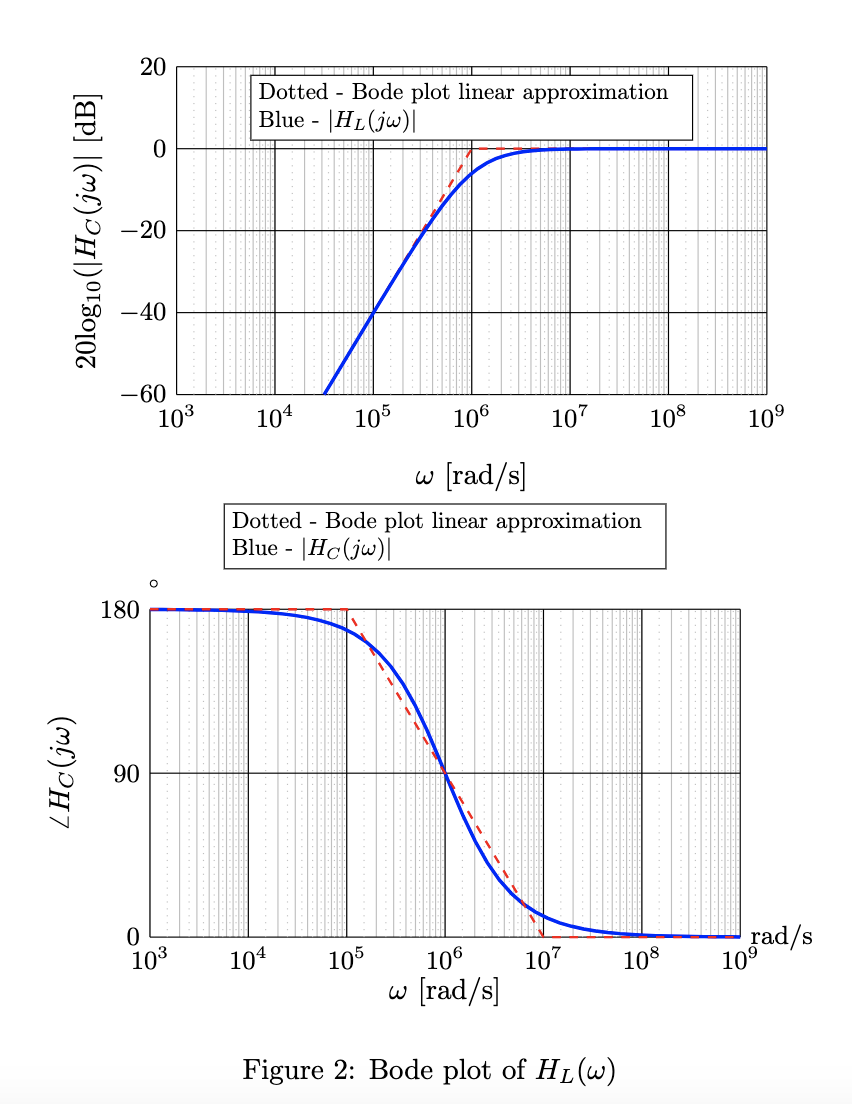
\includegraphics[width=0.8\textwidth]{\bank/transfer/figures/hl.png}
  % \caption{Bode plot of $H_L(\omega)$}
   \end{figure}
  % \begin{figure}[H]
    \centering
    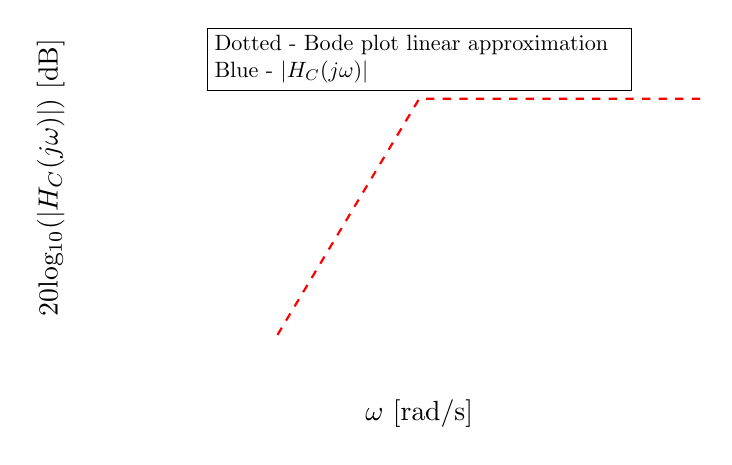
\begin{tikzpicture}[
        gnuplot def/.append style={prefix={}},
    ]
     \tikzset{
     semilog lines/.style={black},
     semilog lines 2/.style={gray!50},
     semilog half lines/.style={gray!50, dotted},
     semilog label x/.style={below,font=\small},
     semilog label y/.style={above,font=\small} }
     
    \begin{scope}[xscale=6/5,yscale=4/80]
    
    % y axis step
    \OrdBode{20}
    
    % Semilog grid
    \semilog*{3}{9}{-60}{20}
    % \BodeGraph[red!80, dashed]{3:9}{\POAmpAsymp{1}{0.000001})+\POAmpAsymp{1}{0.000001})}
    \draw [red, dashed, thick] (4.5,-60) -- (6,0) -- (9,0);
    \BodeGraph{4.5:9} {-(\PIAmp{1}{0.000001})-(\PIAmp{1}{0.000001})}
    % \BodeGraph[red!80, dashed]{-2:3}{\POAmpAsymp{100}{0.1}}
    % {20*log10(abs(sqrt(1+(0.1*10**t)**2)/sqrt(1+(100*10**t)**2)))}
    % {-\POAmp{1}{0.1}} flips over x axis center flat then down or up
    % {-\PIAmp{1}{0.1})} down or up then flat
    \node
        [rectangle, draw, fill=white, text width = 6.5cm, scale=0.8] 
        at (6,10) {Dotted - Bode plot linear approximation \\ Blue - $|H_C(j\omega)|$};
    \node[rotate=0] at (6, -80) {$\omega$ [rad/s]};
    \node[rotate=90] at (2.1, -20) {20log$_{10}(|H_C(j\omega)|)$ [dB]};
    \end{scope}
    \end{tikzpicture}
    
    \begin{tikzpicture}[
        gnuplot def/.append style={prefix={}},
    ]
     \tikzset{
     semilog lines/.style={black},
     semilog lines 2/.style={gray!50},
     semilog half lines/.style={gray!50, dotted},
     semilog label x/.style={below,font=\small},
     semilog label y/.style={above,font=\small} }
     
    \begin{scope}[xscale=6/5,yscale=4/180]
    
    % y axis step
    \OrdBode{90}
    \UniteDegre
    % Semilog grid
    \semilog*{3}{9}{0}{180}
    % \BodeGraph[red!80, dashed]{3:9}{\POArgAsymp{1}{0.000001})}
    \BodeGraph{3:9} {-(\PIArg{1}{0.000001})-(\PIArg{1}{0.000001})}
    \draw [red, dashed, thick] (3,180) -- (5,180) -- (7,0) -- (9,0);
    % \BodeGraph[red!80, dashed]{-2:3}{\POAmpAsymp{100}{0.1}}
    % {20*log10(abs(sqrt(1+(0.1*10**t)**2)/sqrt(1+(100*10**t)**2)))}
    % {-\POAmp{1}{0.1}} flips over x axis center flat then down or up
    % {-\PIAmp{1}{0.1})} down or up then flat
    \node
        [rectangle, draw, fill=white, text width = 6.5cm, scale=0.8] 
        at (6,220) {Dotted - Bode plot linear approximation \\ Blue - $|H_C(j\omega)|$};
    \node[rotate=0] at (6, -30) {$\omega$ [rad/s]};
    \node[rotate=90] at (2.1, 90) {$\angle{H_{C}(j\omega)}$};
    
    \end{scope}
    \end{tikzpicture}
    \caption{Bode plot of $H_L(\omega)$}
    \end{figure}
  
$H_R(\omega)$:

Poles: same as others, 2 poles at $10^6 \si{\radian\per\second}$.

Zeros: Like $H_L(\omega)$, it has a zero at \SI{0}{\radian\per\second}, but this time there is only 1.

This creates a bandpass filter. To find the peak magnitude, we look at the first asymptote. Before $\omega_c$, the only pole or zero that affects $|H(\omega)|$ is the zero at \SI{0}{\radian\per\second}:
\[|H_{R}(\omega \leq \omega_c)|= |j\omega RC|\]
Plugging in $\omega=\omega_c$ will give us the peak value of the transfer function:
\begin{align*}
|H_{R}(\omega = \omega_c)|&= |j\omega_c RC|=\left|\frac{jRC}{\sqrt{LC}}\right| = \left|\frac{jR\sqrt{C}}{\sqrt{L}}\right| \\
 |H_{R}(\omega = \omega_c)|&= \frac{\SI{2000}{\ohm}\sqrt{10^{-9}\si{\farad}}}{\sqrt{10^{-3}\si{\henry}}} = 2
\end{align*}

   \begin{figure}[H]\centering
   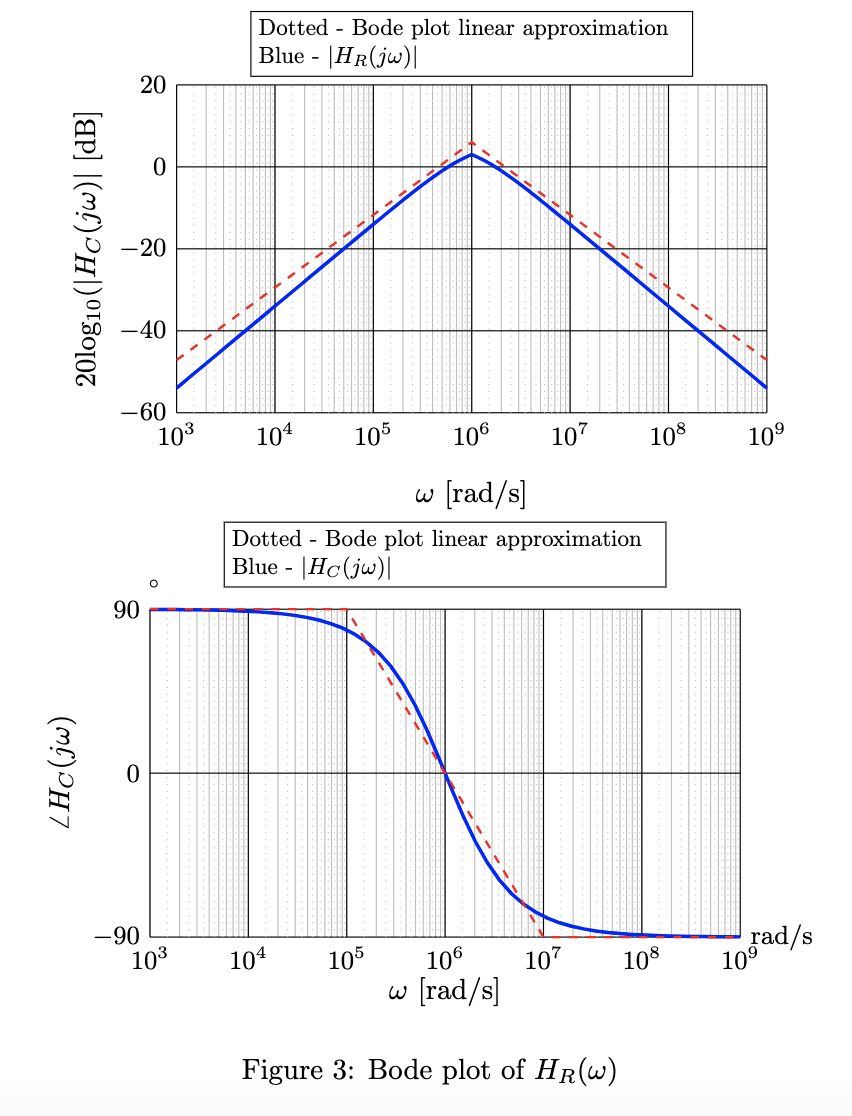
\includegraphics[width=0.8\textwidth]{\bank/transfer/figures/hr.png}
  % \caption{Bode plot of $H_R(\omega)$}
   \end{figure}
  % \begin{figure}[H]
    \centering
    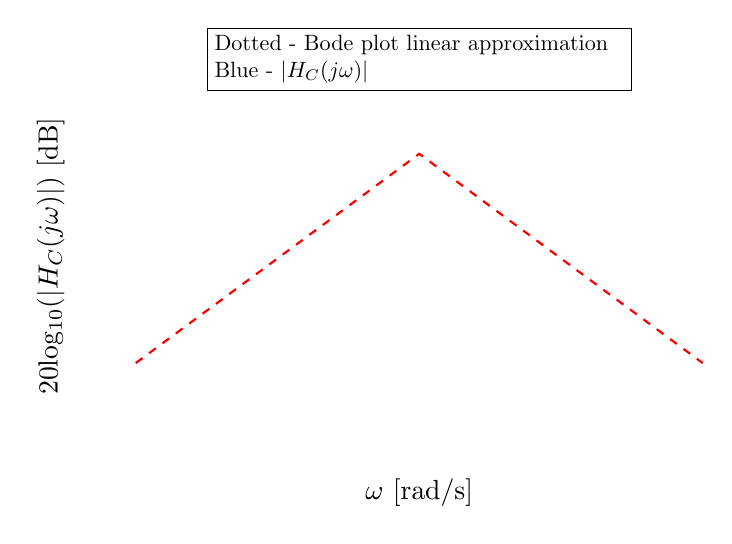
\begin{tikzpicture}[
        gnuplot def/.append style={prefix={}},
    ]
     \tikzset{
     semilog lines/.style={black},
     semilog lines 2/.style={gray!50},
     semilog half lines/.style={gray!50, dotted},
     semilog label x/.style={below,font=\small},
     semilog label y/.style={above,font=\small} }
     
    \begin{scope}[xscale=6/5,yscale=4/80]
    
    % y axis step
    \OrdBode{20}
    
    % Semilog grid
    \semilog*{3}{9}{-60}{20}
    % \BodeGraph[red!80, dashed]{3:9}{\POAmpAsymp{1}{0.000001})+\POAmpAsymp{1}{0.000001})}
    \draw [red, dashed, thick] (3,-47.16) -- (6,6) -- (9,-47.17);
    \BodeGraph{6:9} {\POAmp{2}{0.000001}}
    \BodeGraph{3:6} {-(\PIAmp{0.5}{0.000001})}
    % \BodeGraph{3:9}{-(\PIDAmp{0.5}{0.08}{0.000001})}
    
    % \BodeGraph[red!80, dashed]{-2:3}{\POAmpAsymp{100}{0.1}}
    % {20*log10(abs(sqrt(1+(0.1*10**t)**2)/sqrt(1+(100*10**t)**2)))}
    % {-\POAmp{1}{0.1}} flips over x axis center flat then down or up
    % {-\PIAmp{1}{0.1})} down or up then flat
    \node
        [rectangle, draw, fill=white, text width = 6.5cm, scale=0.8] 
        at (6,30) {Dotted - Bode plot linear approximation \\ Blue - $|H_C(j\omega)|$};
    \node[rotate=0] at (6, -80) {$\omega$ [rad/s]};
    \node[rotate=90] at (2.1, -20) {20log$_{10}(|H_C(j\omega)|)$ [dB]};
    \end{scope}
    \end{tikzpicture}
    
    \begin{tikzpicture}[
        gnuplot def/.append style={prefix={}},
    ]
     \tikzset{
     semilog lines/.style={black},
     semilog lines 2/.style={gray!50},
     semilog half lines/.style={gray!50, dotted},
     semilog label x/.style={below,font=\small},
     semilog label y/.style={above,font=\small} }
     
    \begin{scope}[xscale=6/5,yscale=4/180]
    
    % y axis step
    \OrdBode{90}
    \UniteDegre
    % Semilog grid
    \semilog*{3}{9}{-90}{90}
    % \BodeGraph[red!80, dashed]{3:9}{\POArgAsymp{1}{0.000001})}
    \BodeGraph{3:9} {90+(-(\PDArg{1}{0.000001}))-(\PDArg{1}{0.000001})}
    \draw [red, dashed, thick] (3,90) -- (5,90) -- (7,-90) -- (9,-90);
    % \BodeGraph[red!80, dashed]{-2:3}{\POAmpAsymp{100}{0.1}}
    % {20*log10(abs(sqrt(1+(0.1*10**t)**2)/sqrt(1+(100*10**t)**2)))}
    % {-\POAmp{1}{0.1}} flips over x axis center flat then down or up
    % {-\PIAmp{1}{0.1})} down or up then flat
    \node
        [rectangle, draw, fill=white, text width = 6.5cm, scale=0.8] 
        at (6,120) {Dotted - Bode plot linear approximation \\ Blue - $|H_C(j\omega)|$};
    \node[rotate=0] at (6, -120) {$\omega$ [rad/s]};
    \node[rotate=90] at (2.1, 0) {$\angle{H_{C}(j\omega)}$};
    
    \end{scope}
    \end{tikzpicture}
    \caption{Bode plot of $H_R(\omega)$}
    \end{figure}
  
}

\qitem \textbf{(Practice) Draw the Bode plot of $H_R(\omega)$ two more times, but change $R$ to be $\SI{20}{\ohm}$, then $\SI{200}{\kilo\ohm}$.}

\sol{

Looking back at our solution in part (e), the only difference is the peak value of $H(\omega)$. Plugging the new resistor values in, we get:

\begin{align*}
R = \SI{20}{\ohm} \to |H(\omega_c)| &= \frac{20\sqrt{10^{-9}}}{\sqrt{10^{-3}}};  \\
R = \SI{200}{\kilo\ohm} \to |H(\omega_c)| &= \frac{2 \cdot 10^5\sqrt{10^{-9}}}{\sqrt{10^{-3}}}.
\end{align*}

Every other part of the Bode plot is the same as the plot in part (e).
  \begin{figure}[H]\centering
  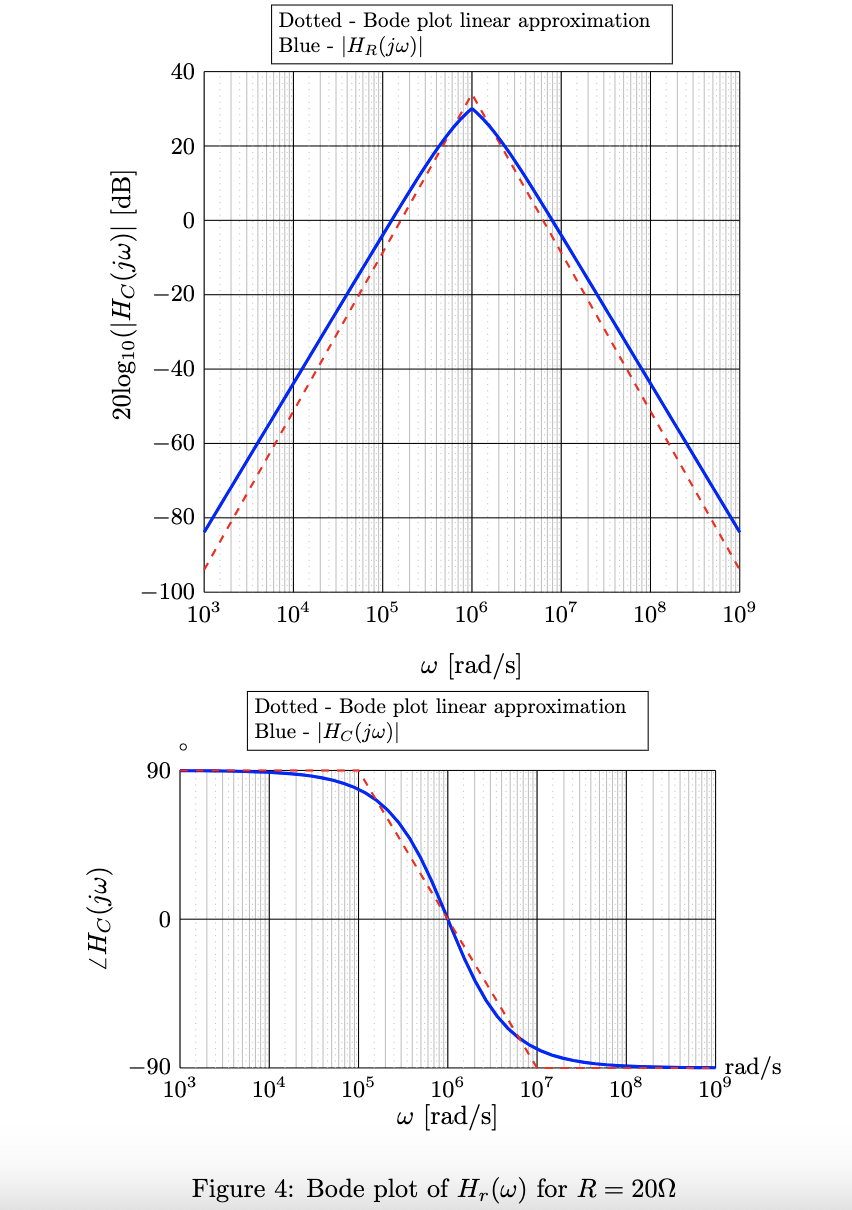
\includegraphics[width=0.8\textwidth]{\bank/transfer/figures/hr_20.png}
  % \caption{Bode plot of $H_R(\omega)$ for $R = \SI{20}{\ohm}$}
  \end{figure}
  
    \begin{figure}[H]\centering
  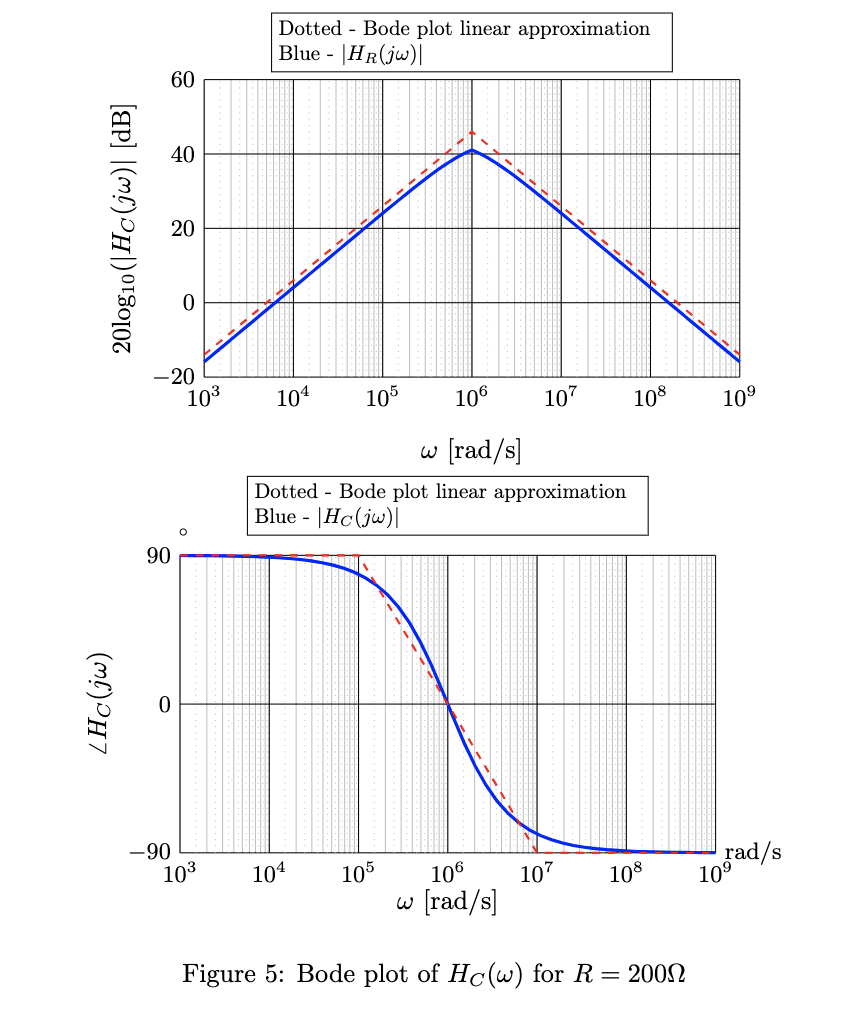
\includegraphics[width=0.8\textwidth]{\bank/transfer/figures/hr_200.png}
  % \caption{Bode plot of $H_R(\omega)$ for $R = \SI{200}{\kilo\ohm}$}
  \end{figure}

  % \begin{figure}[H]
    \centering
    \begin{tikzpicture}[
        gnuplot def/.append style={prefix={}},
    ]
     \tikzset{
     semilog lines/.style={black},
     semilog lines 2/.style={gray!50},
     semilog half lines/.style={gray!50, dotted},
     semilog label x/.style={below,font=\small},
     semilog label y/.style={above,font=\small} }
     
    \begin{scope}[xscale=6/5,yscale=4/80]
    
    % y axis step
    \OrdBode{20}
    
    % Semilog grid
    \semilog*{3}{9}{-100}{40}
    % \BodeGraph[red!80, dashed]{3:9}{\POAmpAsymp{1}{0.000001})+\POAmpAsymp{1}{0.000001})}
    \draw [red, dashed, thick] (3,-93.98) -- (6,33.98) -- (9,-93.98);
    \BodeGraph{6:9} {(\POAmp{8}{0.000001}+\POAmp{8}{0.000001})}
    \BodeGraph{3:6} {-((\PIAmp{0.125}{0.000001})+(\PIAmp{0.125}{0.000001}))}
    % \BodeGraph{3:9}{-(\PIDAmp{0.5}{0.08}{0.000001})}
    
    % \BodeGraph[red!80, dashed]{-2:3}{\POAmpAsymp{100}{0.1}}
    % {20*log10(abs(sqrt(1+(0.1*10**t)**2)/sqrt(1+(100*10**t)**2)))}
    % {-\POAmp{1}{0.1}} flips over x axis center flat then down or up
    % {-\PIAmp{1}{0.1})} down or up then flat
    \node
        [rectangle, draw, fill=white, text width = 6.5cm, scale=0.8] 
        at (6,50) {Dotted - Bode plot linear approximation \\ Blue - $|H_C(j\omega)|$};
    \node[rotate=0] at (6, -120) {$\omega$ [rad/s]};
    \node[rotate=90] at (2.1, -20) {20log$_{10}(|H_C(j\omega)|)$ [dB]};
    \end{scope}
    \end{tikzpicture}
    
    \begin{tikzpicture}[
        gnuplot def/.append style={prefix={}},
    ]
     \tikzset{
     semilog lines/.style={black},
     semilog lines 2/.style={gray!50},
     semilog half lines/.style={gray!50, dotted},
     semilog label x/.style={below,font=\small},
     semilog label y/.style={above,font=\small} }
     
    \begin{scope}[xscale=6/5,yscale=4/180]
    
    % y axis step
    \OrdBode{90}
    \UniteDegre
    % Semilog grid
    \semilog*{3}{9}{-90}{90}
    % \BodeGraph[red!80, dashed]{3:9}{\POArgAsymp{1}{0.000001})}
    \BodeGraph{3:9} {90+(-(\PDArg{1}{0.000001}))-(\PDArg{1}{0.000001})}
    \draw [red, dashed, thick] (3,90) -- (5,90) -- (7,-90) -- (9,-90);
    % \BodeGraph[red!80, dashed]{-2:3}{\POAmpAsymp{100}{0.1}}
    % {20*log10(abs(sqrt(1+(0.1*10**t)**2)/sqrt(1+(100*10**t)**2)))}
    % {-\POAmp{1}{0.1}} flips over x axis center flat then down or up
    % {-\PIAmp{1}{0.1})} down or up then flat
    \node
        [rectangle, draw, fill=white, text width = 6.5cm, scale=0.8] 
        at (6,120) {Dotted - Bode plot linear approximation \\ Blue - $|H_C(j\omega)|$};
    \node[rotate=0] at (6, -120) {$\omega$ [rad/s]};
    \node[rotate=90] at (2.1, 0) {$\angle{H_{C}(j\omega)}$};
    
    \end{scope}
    \end{tikzpicture}
    \caption{Bode plot of $H_r(\omega)$ for $R=20 \Omega$}
    \end{figure}

  % \begin{figure}[H]
    \centering
    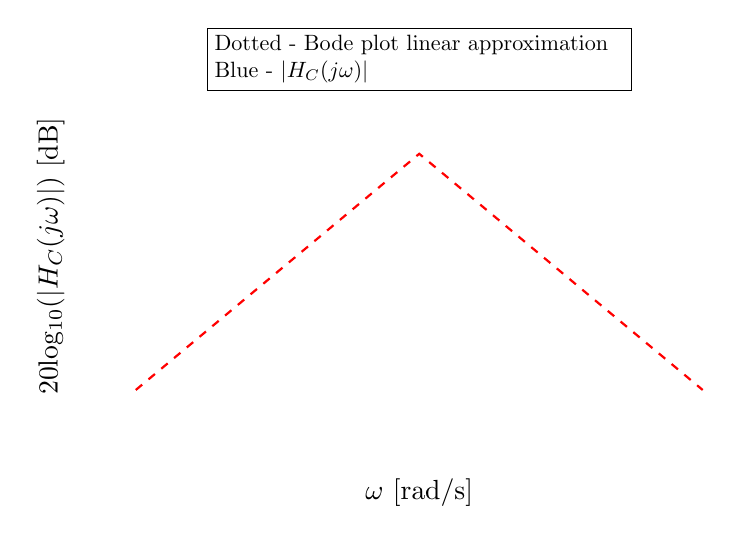
\begin{tikzpicture}[
        gnuplot def/.append style={prefix={}},
    ]
     \tikzset{
     semilog lines/.style={black},
     semilog lines 2/.style={gray!50},
     semilog half lines/.style={gray!50, dotted},
     semilog label x/.style={below,font=\small},
     semilog label y/.style={above,font=\small} }
     
    \begin{scope}[xscale=6/5,yscale=4/80]
    
    % y axis step
    \OrdBode{20}
    
    % Semilog grid
    \semilog*{3}{9}{-20}{60}
    % \BodeGraph[red!80, dashed]{3:9}{\POAmpAsymp{1}{0.000001})+\POAmpAsymp{1}{0.000001})}
    \draw [red, dashed, thick] (3,-14) -- (6,46) -- (9,-14);
    \BodeGraph{6:9} {\POAmp{160}{0.000001}}
    \BodeGraph{3:6} {-(\PIAmp{0.00625}{0.000001})}
    % \BodeGraph{3:9}{-(\PIDAmp{0.5}{0.08}{0.000001})}
    
    % \BodeGraph[red!80, dashed]{-2:3}{\POAmpAsymp{100}{0.1}}
    % {20*log10(abs(sqrt(1+(0.1*10**t)**2)/sqrt(1+(100*10**t)**2)))}
    % {-\POAmp{1}{0.1}} flips over x axis center flat then down or up
    % {-\PIAmp{1}{0.1})} down or up then flat
    \node
        [rectangle, draw, fill=white, text width = 6.5cm, scale=0.8] 
        at (6,70) {Dotted - Bode plot linear approximation \\ Blue - $|H_C(j\omega)|$};
    \node[rotate=0] at (6, -40) {$\omega$ [rad/s]};
    \node[rotate=90] at (2.1, 20) {20log$_{10}(|H_C(j\omega)|)$ [dB]};
    \end{scope}
    \end{tikzpicture}
    
    \begin{tikzpicture}[
        gnuplot def/.append style={prefix={}},
    ]
     \tikzset{
     semilog lines/.style={black},
     semilog lines 2/.style={gray!50},
     semilog half lines/.style={gray!50, dotted},
     semilog label x/.style={below,font=\small},
     semilog label y/.style={above,font=\small} }
     
    \begin{scope}[xscale=6/5,yscale=4/180]
    
    % y axis step
    \OrdBode{90}
    \UniteDegre
    % Semilog grid
    \semilog*{3}{9}{-90}{90}
    % \BodeGraph[red!80, dashed]{3:9}{\POArgAsymp{1}{0.000001})}
    \BodeGraph{3:9} {90+(-(\PDArg{1}{0.000001}))-(\PDArg{1}{0.000001})}
    \draw [red, dashed, thick] (3,90) -- (5,90) -- (7,-90) -- (9,-90);
    % \BodeGraph[red!80, dashed]{-2:3}{\POAmpAsymp{100}{0.1}}
    % {20*log10(abs(sqrt(1+(0.1*10**t)**2)/sqrt(1+(100*10**t)**2)))}
    % {-\POAmp{1}{0.1}} flips over x axis center flat then down or up
    % {-\PIAmp{1}{0.1})} down or up then flat
    \node
        [rectangle, draw, fill=white, text width = 6.5cm, scale=0.8] 
        at (6,120) {Dotted - Bode plot linear approximation \\ Blue - $|H_C(j\omega)|$};
    \node[rotate=0] at (6, -120) {$\omega$ [rad/s]};
    \node[rotate=90] at (2.1, 0) {$\angle{H_{C}(j\omega)}$};
    
    \end{scope}
    \end{tikzpicture}
    \caption{Bode plot of $H_C(\omega)$ for $R=200\Omega$}
    \end{figure}
  
}

% \qitem \textbf{Find $\omega_{c1}$ and $\omega_{c2}$ of $H_R(\omega)$ for $R = \SI{20}{\ohm}$, $R=\SI{2}{\kilo\ohm}$, and $R= \SI{200}{\kilo\ohm}$.}

% \sol{

% While we said that the corner frequencies were at $10^6 \si{\radian\per\second}$ in part (e), that was only for the Bode plot approximation. $10^6 \si{\radian\per\second}$ is actually the center frequency. To get the corner frequencies, we need to find the values of $\omega$ where $|H_R(\omega)| = \frac{1}{\sqrt{2}}$.
% \begin{align*}
% \omega_{c1,c2}&=\sqrt{\left(\frac{R}{2L}\right)^2+\frac{1}{LC}} \pm \frac{R}{2L} \\
% R &= \SI{20}{\ohm} \to \omega_{c1} = \SI{9.9005e5}{\radian\per\second}, \omega_{c2} = \SI{1.01e6}{\radian\per\second} \\
% R &= \SI{2000}{\ohm} \to \omega_{c1} = \SI{4.1421e5}{\radian\per\second}, \omega_{c2} = \SI{2.4142e6}{\radian\per\second} \\
% R &= \SI{200000}{\ohm} \to \omega_{c1} = \SI{0.05e5}{\radian\per\second}, \omega_{c2} = \SI{2e8}{\radian\per\second}
% \end{align*}
% }

% \qitem \textbf{Which of the three values of $R$ gives the largest bandwidth? Which gives the highest $Q$?}

% \sol{

% \begin{align*}
% BW &= \omega_{c2}-\omega_{c1} \\
% BW(\SI{20}{\ohm}) &= \SI{2e4}{\radian\per\second} \\
% BW(2000\Omega) &= \SI{2e6}{\radian\per\second} \\ 
% BW(200000\Omega) &= \SI{2e8}{\radian\per\second}
% \end{align*}
% $R=\SI{200}{\kilo\ohm}$ gives the highest bandwidth.

% \begin{align*}
% Q = \frac{\omega_0}{BW} &= \frac{10^6 \si{\radian\per\second}}{BW} \\
% Q(\SI{20}{\ohm}) &= 50 \\
% Q(2000\Omega) &= 0.5 \\ 
% Q(200000\Omega) &=  0.005
% \end{align*}
% $R=\SI{20}{\ohm}$ gives the highest $Q$.

% }

\begin{comment}
\qitem Given the actual frequency response of $H_R(\omega)$ for $R = \SI{20}{\ohm}$, $R=\SI{2}{\kilo\ohm}$, and $R= \SI{200}{\kilo\ohm}$, what is different between the Bode plots and the actual responses? Label on each graph what type of damping the circuit experiences.

  \begin{figure}[H]\centering
  \includegraphics[width=0.7\textwidth]{q_rlc_bode/q1i_20.png}
  \caption{$R=\SI{20}{\ohm}$ frequency response}
  \end{figure}
  \begin{figure}[H]\centering
  \includegraphics[width=0.7\textwidth]{q_rlc_bode/q1i_2k.png}
  \caption{$R=\SI{2}{\kilo\ohm}$ frequency response}
  \end{figure}
  \begin{figure}[H]\centering
  \includegraphics[width=0.7\textwidth]{q_rlc_bode/q1i_200k.png}
  \caption{$R=\SI{200}{\kilo\ohm}$ frequency response}
  \end{figure}

\sol{
  
The three frequency responses are now different from each other. The peak gain for each case is now \SI{0}{\decibel}, instead of varying. This is because the Bode approximation ignores the $\omega$ term in the quadratic pole equation. However, the different values of $\xi$ affect the gain in the passband significantly. The passband of each one corresponds to the bandwidth of the filter. The phase no longer is a constant $\frac{\ang{-90}}{\text{dec}}$ drop; it now depends on the resistor value. The frequency responses are different because the Bode plots only look at the asymptotes of the frequency response; it doesn't take into account things like $Q$ or bandwidth. For second order and higher transfer functions, Bode plots are not always the most accurate.

To determine the damping, we can use the same equations in the past:
\begin{align*}
\alpha&=\frac{R}{2L} \\
\omega_0 &= \frac{1}{\sqrt{LC}}
\end{align*}
We know the system is critically damped when $\alpha = \omega_0$.

Using substitution, we get
\[R = 2\sqrt{\frac{L}{C}} = \SI{2}{\kilo\ohm}\]
Since $R$ is directly proportional to $\alpha$, we know that if $R<\SI{2}{\kilo\ohm}$, then the system is underdamped, while if $R>\SI{2}{\kilo\ohm}$, then the system is overdamped.
\begin{align*}
R&= \SI{20}{\ohm} \to \text{underdamped} \\
R&= \SI{2}{\kilo\ohm} \to \text{critically damped} \\
R&= \SI{200}{\kilo\ohm} \to \text{overdamped} \\
\end{align*}

Another way to think about damping is to look at the zeros of the quadratic. Back at the differential equations, we saw that the system was underdamped if the solution to the second order equation was complex, it was critically damped if the solutions were the same, and it was overdamped if the solutions were purely real. These conditions still hold for the quadratic pole.

\[\omega = \frac{-\frac{2\xi}{\omega_0}\pm \sqrt{\left(\frac{2\xi}{\omega_0}\right)^2-\frac{4}{\omega_0^2}}}{2\frac{1}{\omega_0^2}}\]
The determining factor on whether $\omega$ is complex is the square root term.
\[\sqrt{\frac{4\xi^2}{\omega_0}-\frac{4}{\omega_0}}=\sqrt{\frac{4}{\omega_0}(\xi^2-1)}\]
If $\xi^2 \leq 1$, then $\omega$ will be complex, which means that the system is underdamped. If $\xi^2 = 1$, then the square root term will be zero, which means that $\omega$ will have repeated roots. This corresponds to a critically damped system. Finally, if $\xi^2 \geq 1$, then the square root term is real and the roots of $\omega$ are both real, which means that this is an overdamped system. By taking the square root of each side, we can say that:
\begin{align*}
|\xi| &\leq 1 \to \text{ Underdamped} \\
|\xi| &= 1 \to \text{ Critically damped} \\
|\xi| &\geq 1 \to \text{ Overdamped}
\end{align*}
Looking back at our transfer function $H_R(\omega)$, we see that
\[\xi = \frac{R\sqrt{C}}{2\sqrt{L}}\]
Plugging into the conditions and isolating $R$, we get
\begin{align*}
|R| &\leq \left|\frac{2\sqrt{L}}{\sqrt{C}}\right| \to \text{ Underdamped} \\
|R| &= \left|\frac{2\sqrt{L}}{\sqrt{C}}\right| \to \text{ Critically damped} \\
|R| &\geq \left|\frac{2\sqrt{L}}{\sqrt{C}}\right| \to \text{ Overdamped} \\
\end{align*}

}
\end{comment}
 
\end{enumerate}

